\documentclass{beamer}
\usetheme{metropolis} % A modern theme with clean design
\usecolortheme{seagull} % Soft, professional color scheme
\usepackage{graphicx}
\usepackage{booktabs}
\usepackage{xcolor}

% Define custom colors
\definecolor{darkblue}{RGB}{0, 51, 102}
\definecolor{darkred}{RGB}{153, 0, 0}
\definecolor{darkgreen}{RGB}{0, 102, 51}
\definecolor{darkorange}{RGB}{204, 85, 0}

% Set colors for different elements
\setbeamercolor{background canvas}{bg=white}
\setbeamercolor{normal text}{fg=black}
\setbeamercolor{frametitle}{fg=darkblue}
\setbeamercolor{title}{fg=darkred}
\setbeamercolor{section in head/foot}{fg=white, bg=darkgreen}

\title{A High Performance Computing Platform for Big Biological Data Analysis}
\author{Chang-Wei Yeh, Chieh-Wei Huang, Chia-Lee Yang, Yu-Tai Wang}
\institute{National Centre for High-Performance Computing, National Applied Research Laboratories, Hsinchu, Taiwan}
\date{\today}

\begin{document}

\frame{\titlepage}

\begin{frame}{Introduction}
    \begin{itemize}
        \item HPC is increasingly used in biology, especially during the COVID-19 pandemic.
        \item Applications include drug discovery, variant modeling, and antibody-virus interaction analysis.
        \item Challenges include unstructured data and complex access patterns.
    \end{itemize}
\end{frame}

\begin{frame}{Related Work}
    \textbf{HPC in Bioinformatics:}
    \begin{itemize}
        \item Bioinformatics has evolved into a big data science.
        \item Techniques: Sequence alignment, genome assembly, pattern discovery.
        \item High computational demands require HPC resources.
    \end{itemize}
\end{frame}

\begin{frame}{Proposed HPC Platform}
    \textbf{System Overview:}
    \begin{itemize}
        \item Designed for genomic sequencing and protein structure analysis.
        \item Utilizes supercomputers, GPUs, and FPGAs.
        \item Optimized for large-scale biological data processing.
    \end{itemize}
\end{frame}

\begin{frame}{Containerized Workflow Services}
    \begin{itemize}
        \item Enables users to run workflows in isolated environments.
        \item Uses Docker/Singularity containers for reproducibility.
        \item Supports bioinformatics tools like Galaxy.
    \end{itemize}
\end{frame}

\begin{frame}{Heterogeneous Computing Nodes}
    \begin{itemize}
        \item Offers a mix of CPUs, GPUs, and FPGAs.
        \item Optimized for different bioinformatics workloads.
        \item Reduces computation time for genomic analysis.
    \end{itemize}
    \begin{center}
        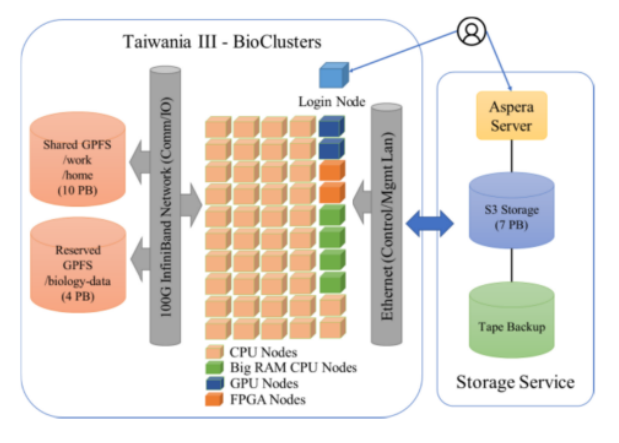
\includegraphics[width=0.7\linewidth]{fig1.png}
    \end{center}
\end{frame}

\begin{frame}{Data Loading Optimization}
    \begin{itemize}
        \item Provides high-speed parallel file systems.
        \item Reduces data migration overhead.
        \item Improves file sharing across research teams.
    \end{itemize}
\end{frame}

\begin{frame}{Scheduling Based on Memory Size}
    \begin{itemize}
        \item Traditional scheduling relies on CPU cores.
        \item NBCF optimizes scheduling based on memory needs.
        \item Reduces queuing time for large-memory applications.
    \end{itemize}
    \begin{center}
        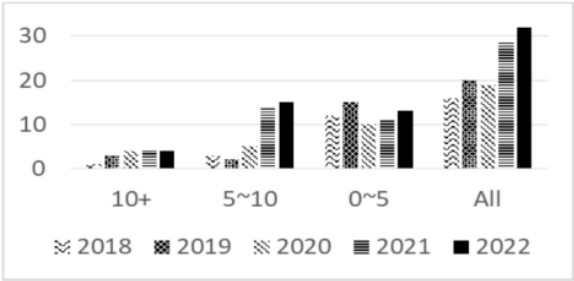
\includegraphics[width=0.7\linewidth]{fig2.png}
    \end{center}
\end{frame}

\begin{frame}{Results}
    \textbf{Impact of NBCF:}
    \begin{itemize}
        \item NBCF supports 30+ institutions and 200-300 researchers annually.
        \item Recognized in over 100 international journal publications.
        \item Impact on genomic and protein analysis research.
    \end{itemize}
\end{frame}

\begin{frame}{Conclusion}
    \textbf{The key takeaways from this research paper are:}
    \begin{itemize}
        \item HPC is crucial for modern biological data analysis.
        \item NBCF enhances computational capabilities for genomic research.
        \item Future improvements aim to further optimize HPC for bioinformatics.
    \end{itemize}
\end{frame}

\begin{frame}{References}
    \begin{itemize}
        \item J. J. Hack and M. E. Papka, "The US high-performance computing consortium in the fight against COVID-19," 2020.
        \item S. Pal et al., "Big data in biology: Challenges and solutions," 2020.
        \item M. N. M. Isa, "High performance reconfigurable architectures for biological sequence alignment," 2013.
    \end{itemize}
\end{frame}

\end{document}
